
\subsubsection{Introduction}
Nearly all the neutrino parameters are already well measured, as shown in Table~\ref{tab:PDGparameters}.                 
In the absence of the matter effect, the amplitude for $\numu\to\nue$ oscillation is given by
\begeq
\langle \nu_e|\nu_\mu(t)\rangle=\Delta_{21}\sin 2\theta_{12}\cos\theta_{23}+e^{-i(\Delta_{31}+\delta)}\sin\Delta_{31}\sin 2\theta_{13}\sin\theta_{23}
\endeq
where we have assumed that $\Delta_{31}\approx \pi/2$ so that $\Delta_{21}\approx \Delta_{31}/30$ is small.  

\begin{eqnarray}
 P(\nu_\mu\to\nu_e)
&=&\sin^2 \theta_{23}\,\sin^22\theta_{13}\,\sin^2 \Delta_{31}\non
 &&\qquad\qquad +\Delta_{21}\sin 2\theta_{13}\sin 2\theta_{12}\,\sin 2 \theta_{23}\sin \Delta_{31} \cos(\Delta_{31} 
 +\delta_{CP})\non
 &&\qquad\qquad\qquad\qquad   +\Delta_{21}^2\cos^2\theta_{23}\sin^2 2\theta_{12} 
 \end{eqnarray}
 where $\Delta_{ij}=\Delta m_{ji}^2 L/(4E)$ and where  $\sin 2\theta_{13}$, $\Delta_{12}$ and 
$|\Delta m_{21}^2/\Delta m_{31}^2|$ are treated as small. In practice, experiments are designed so that oscillations are maximal, i.e. $\Delta_{31}\approx \pi/2$. For ${\overline \nu}_\mu \to {\overline\nu}_e$ the sign of $\delta_{CP}$ is reversed.  Notice that changing $\Delta_{31}$ to $-\Delta_{31}$  and $\delta_{CP}$ to $\pi-\delta_{CP}$ leaves $P$ unchanged so measuring $P(\nu_\mu\to\nu_e)$ and the corresponding probability for $\nubar$ cannot alone determine the hierarchy.  
 
If we adopt as polar coordinates
\begeq
r=\sin 2\theta_{13}; \quad \theta=\delta_{CP}
\endeq
then a result $P_\nu$ for $P(\numu\to\nue)$ gives a circle with radius squared proportional to $P_\nu$.
%\begeq
%A(x^2+y^2)+B(x\cos\Delta_{31}-y\sin\Delta_{31}) + C= P_\nu
%\endeq
%with
%\begeqar
%A&=& \sin^2 \theta_{23}\,\sin^2 \Delta_{31} \non
%B&=&\Delta_{21}\sin 2\theta_{12}\,\sin 2 \theta_{23}\sin \Delta_{31} \non
%C&=&\Delta_{21}^2\cos^2\theta_{23}\sin^2 2\theta_{12} 
%\endeqar
%whose center is at 
%\begeq
%(x_{center},y_{center})=(-\frac B{2A}\cos\Delta_{31},\frac B{2A}\sin\Delta_{31})
%\endeq
%with radius squared
%\begeq
%\frac{P_\nu -C}A +\frac{B^2}{4A^2}=\frac{P_\nu }A \, ,
%\endeq
%where we used the relation $B^2=4AC$.


Similarly, the result $P_\nubar$ for $\numubar\to \nuebar$ gives a circle with a different center and radius squared proportional to $P_\nubar$.
%whose center is at 
%\begeq
%(x_{center},y_{center})=(-\frac B{2A}\cos\Delta_{31},-\frac B{2A}\sin\Delta_{31})
%\endeq
%with radius squared
%\begeq
%\frac{P_\nubar}A .
%\endeq

Perfect measurements of $P(\nu_\mu\to\nu_e)$ and $P(\nubar_\mu\to\nubar_e)$ would give two intersecting circles.  The plots for normal and inverted hierarchies would be mirror images of each other.


When the matter effect is included, the result is 
\begin{eqnarray}
 &&P(\nu_\mu\to\nu_e)
=\sin^2 \theta_{23}\,\sin^22\theta_{13}\,\frac{\sin^2 (1-x)\Delta_{31}}{(1-x)^2}\non
 &&\quad +\frac{\Delta m_{21}^2}{\Delta m_{31}^2}\sin 2\theta_{13}\sin 2\theta_{12}\,\sin 2 \theta_{23}\frac{\sin[(1-x) \Delta_{31}]}{1-x}  \frac{\sin x\Delta_{31}}x\cos(\Delta_{31}+\delta_{CP})\non
 &&\qquad\qquad  +\left(\frac{\Delta m_{21}^2}{\Delta m_{31}^2}\right)^2
 \cos^2\theta_{23}\sin^2 2\theta_{12} \frac{\sin^2( x\Delta_{31})}{x^2} 
 \end{eqnarray}
where $x=2\sqrt 2 G_F N_e E/\Delta m_{31}^2$ and where non-leading terms in $\Delta m_{21}^2/\Delta m_{31}^2$ and $\theta_{13}$ have been neglected.  

%Now the coefficients are given by

%\begeqar
%A&=& \sin^2 \theta_{23}\,\frac{\sin^2 (1-x)\Delta_{31}}{(1-x)^2} \non
%B&=&\frac{\Delta m_{21}^2}{\Delta m_{31}^2}\sin 2\theta_{12}\,\sin 2 \theta_{23}\frac{\sin(1-x) \Delta_{31}}{1-x}\frac{\sin x\Delta_{31}}x \non
%C&=&\left(\frac{\Delta m_{21}^2}{\Delta m_{31}^2}\right)^2
 %\cos^2\theta_{23}\sin^2 2\theta_{12} \frac{\sin^2( x\Delta_{31})}{x^2} 
%\endeqar


For antineutrino scattering, again the sign of $\delta_{CP}$ changes, but also the sign of $x$ is reversed because the effective potential for neutral current scattering of $\nuebar$ is the negative of that for $\nue$.  
 
 
For any given experiment with data for both $P(\nu_\mu\to\nu_e)$ and $P(\nubar_\mu\to\nubar_e)$, we can draw two circles to represent these data.  Of course, in practice the circles would have  thicknesses indicative of the uncertainties  in the measurement.  In addition, a circle could be drawn, with center at the origin, for the measurement of $\sin^2 2\theta_{13}$ from reactor experiments.  Two plots would be made, one on the assumption of normal hierarchy, the other assuming inverted hierarchy.  In at least one of the two there should be a solution where the three circles intersect.  

As we see in the examples below,  the centers of the circles are such that $\delta_{CP}=\pi/2$ and $\delta_{CP}=3\pi/2$ form the extreme situations, making either maximal or minimal separation between the circles.  
 With increasing length $L$, the discriminating power increases as the radii of the circles grow and shrink in the different hierarchies.

\subsubsection{T2K}
T2K runs 295 km from J-PARC in Tokai to Super-Kamiokande.   In Fig.~\ref{fig_four} we see that the low energy of the T2K beam makes it impossible to determine the hierarchy if $\delta_{CP}=\pi/2$, and even for $\delta_{CP}=3\pi/2$, superb precision would be required.
\begin{figure}\begin{center}
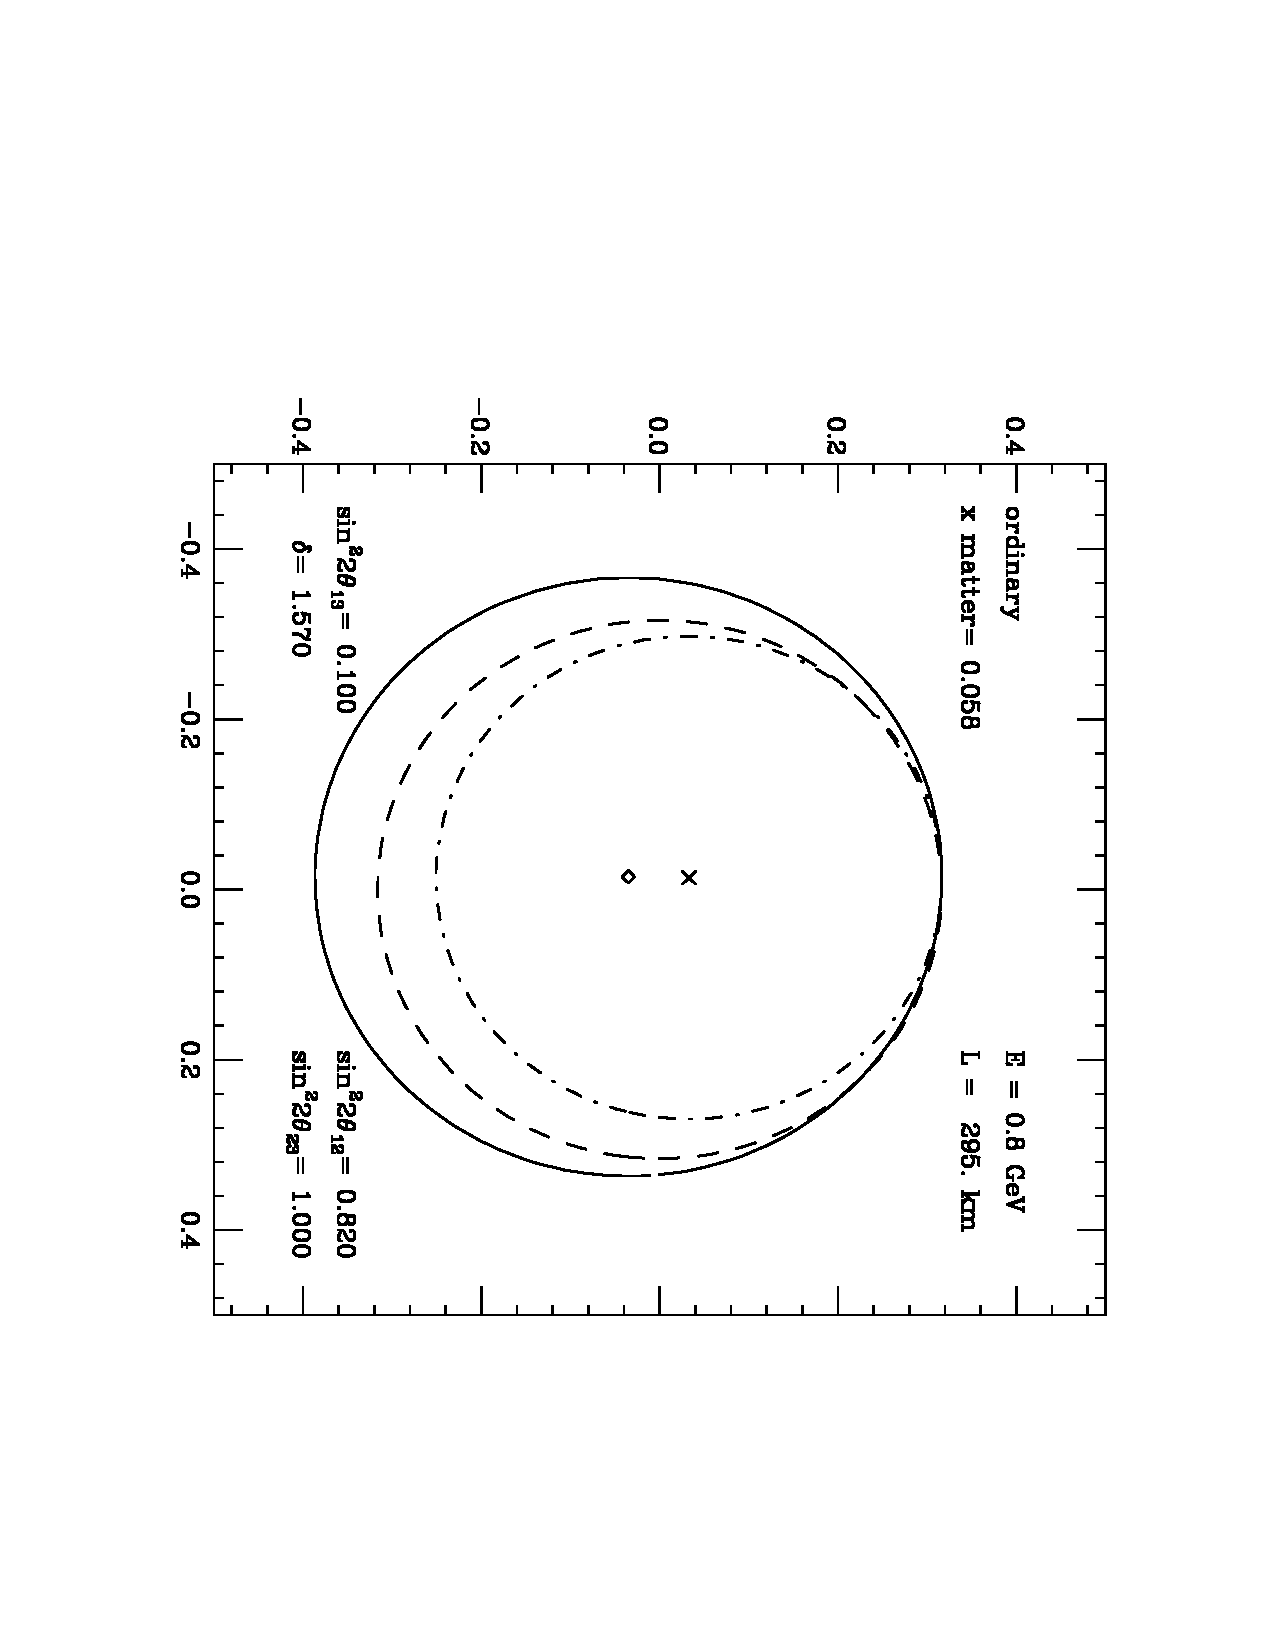
\includegraphics[width=2.75in,angle=90]{RNC/cpv_t2k_pibytwo.pdf}
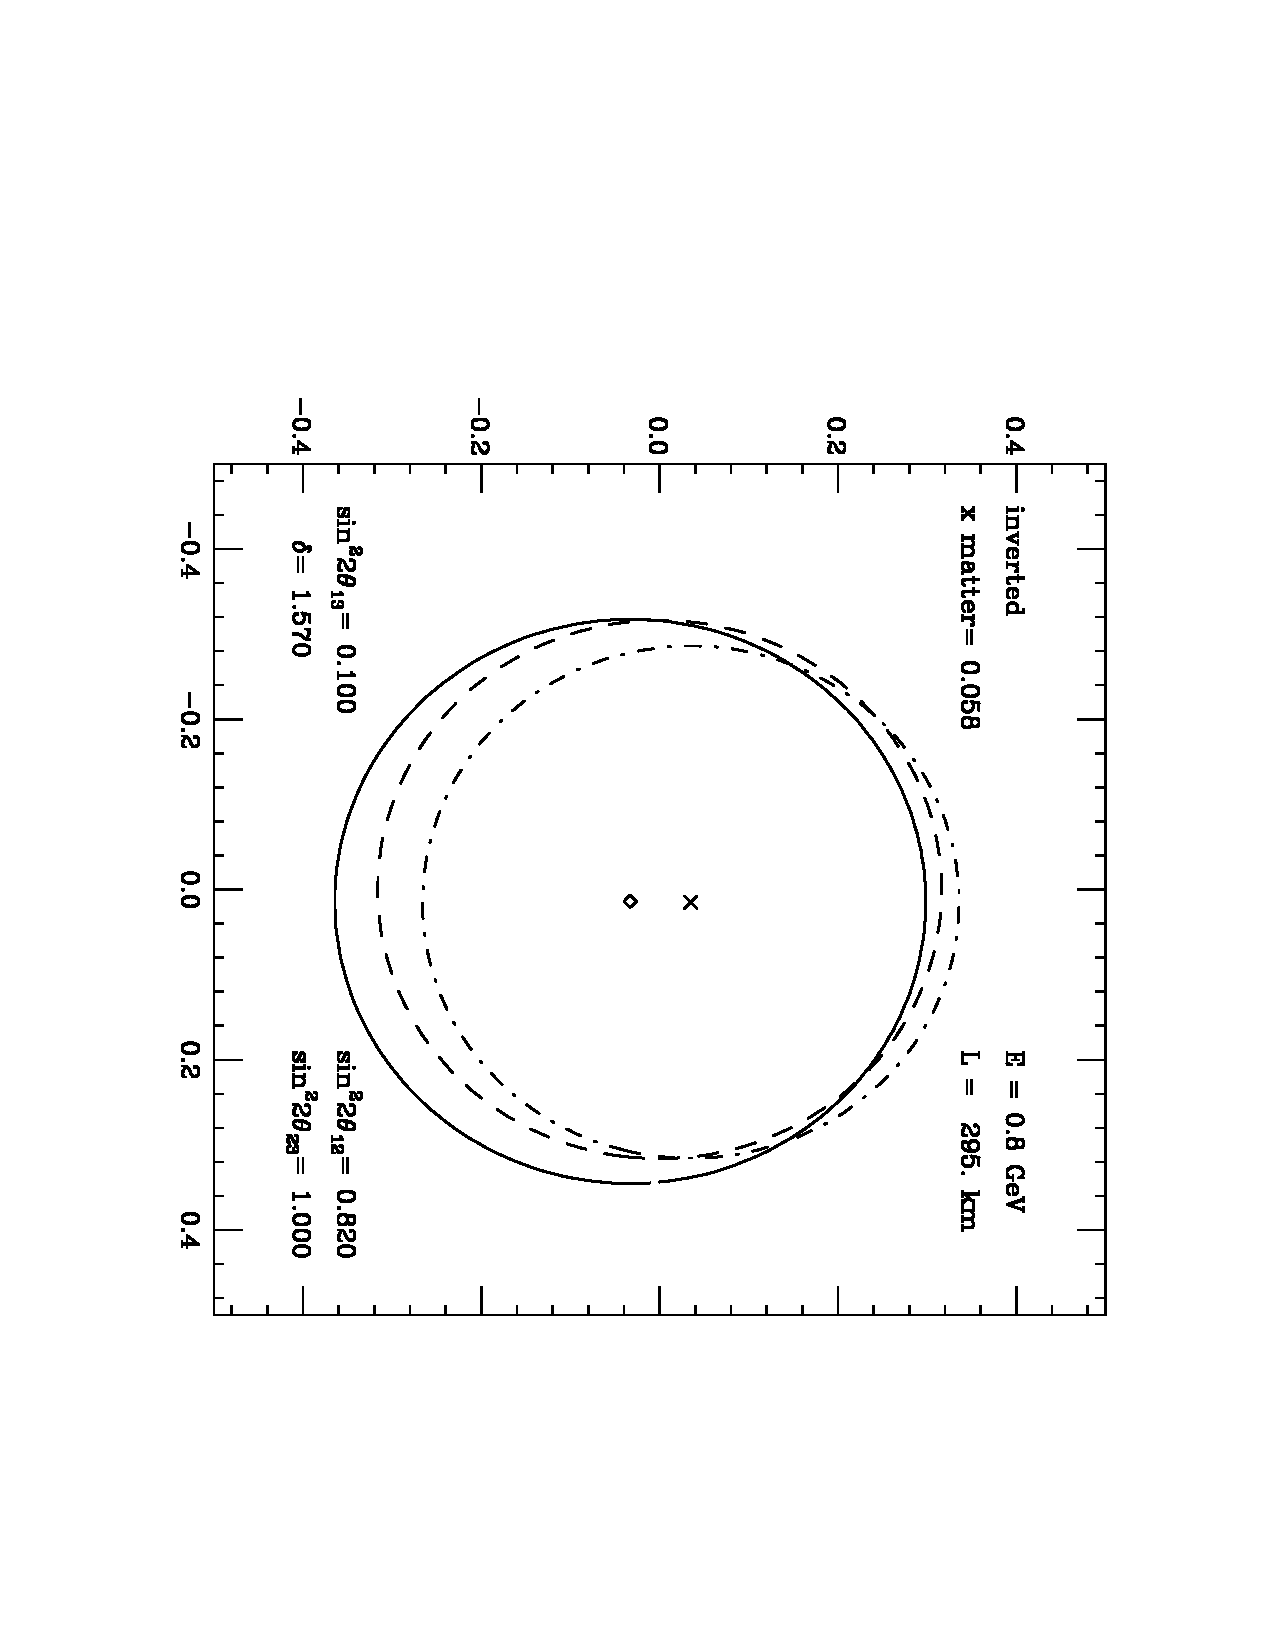
\includegraphics[width=2.75in,angle=90]{RNC/cpv_t2k_pibytwo_inv.pdf}

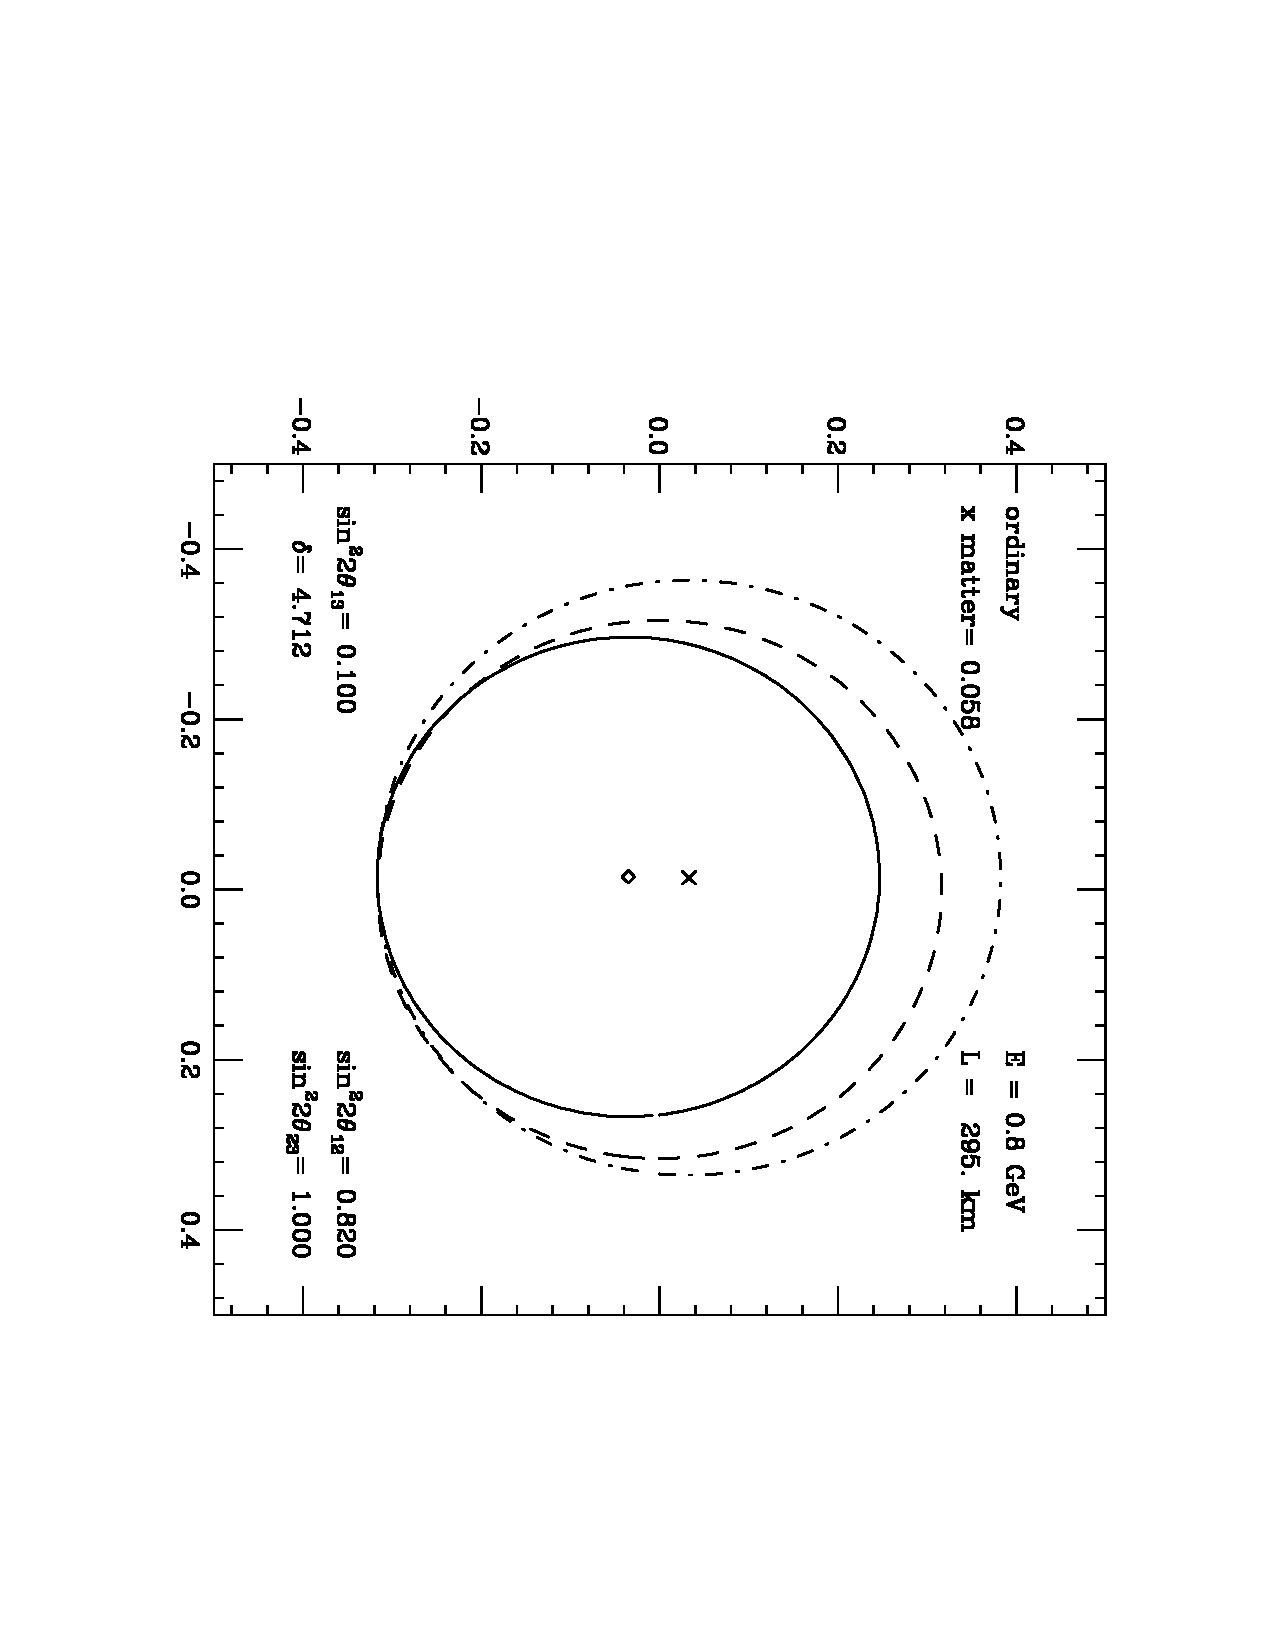
\includegraphics[width=2.75in,angle=90]{RNC/cpv_t2k_threepibytwo.pdf}
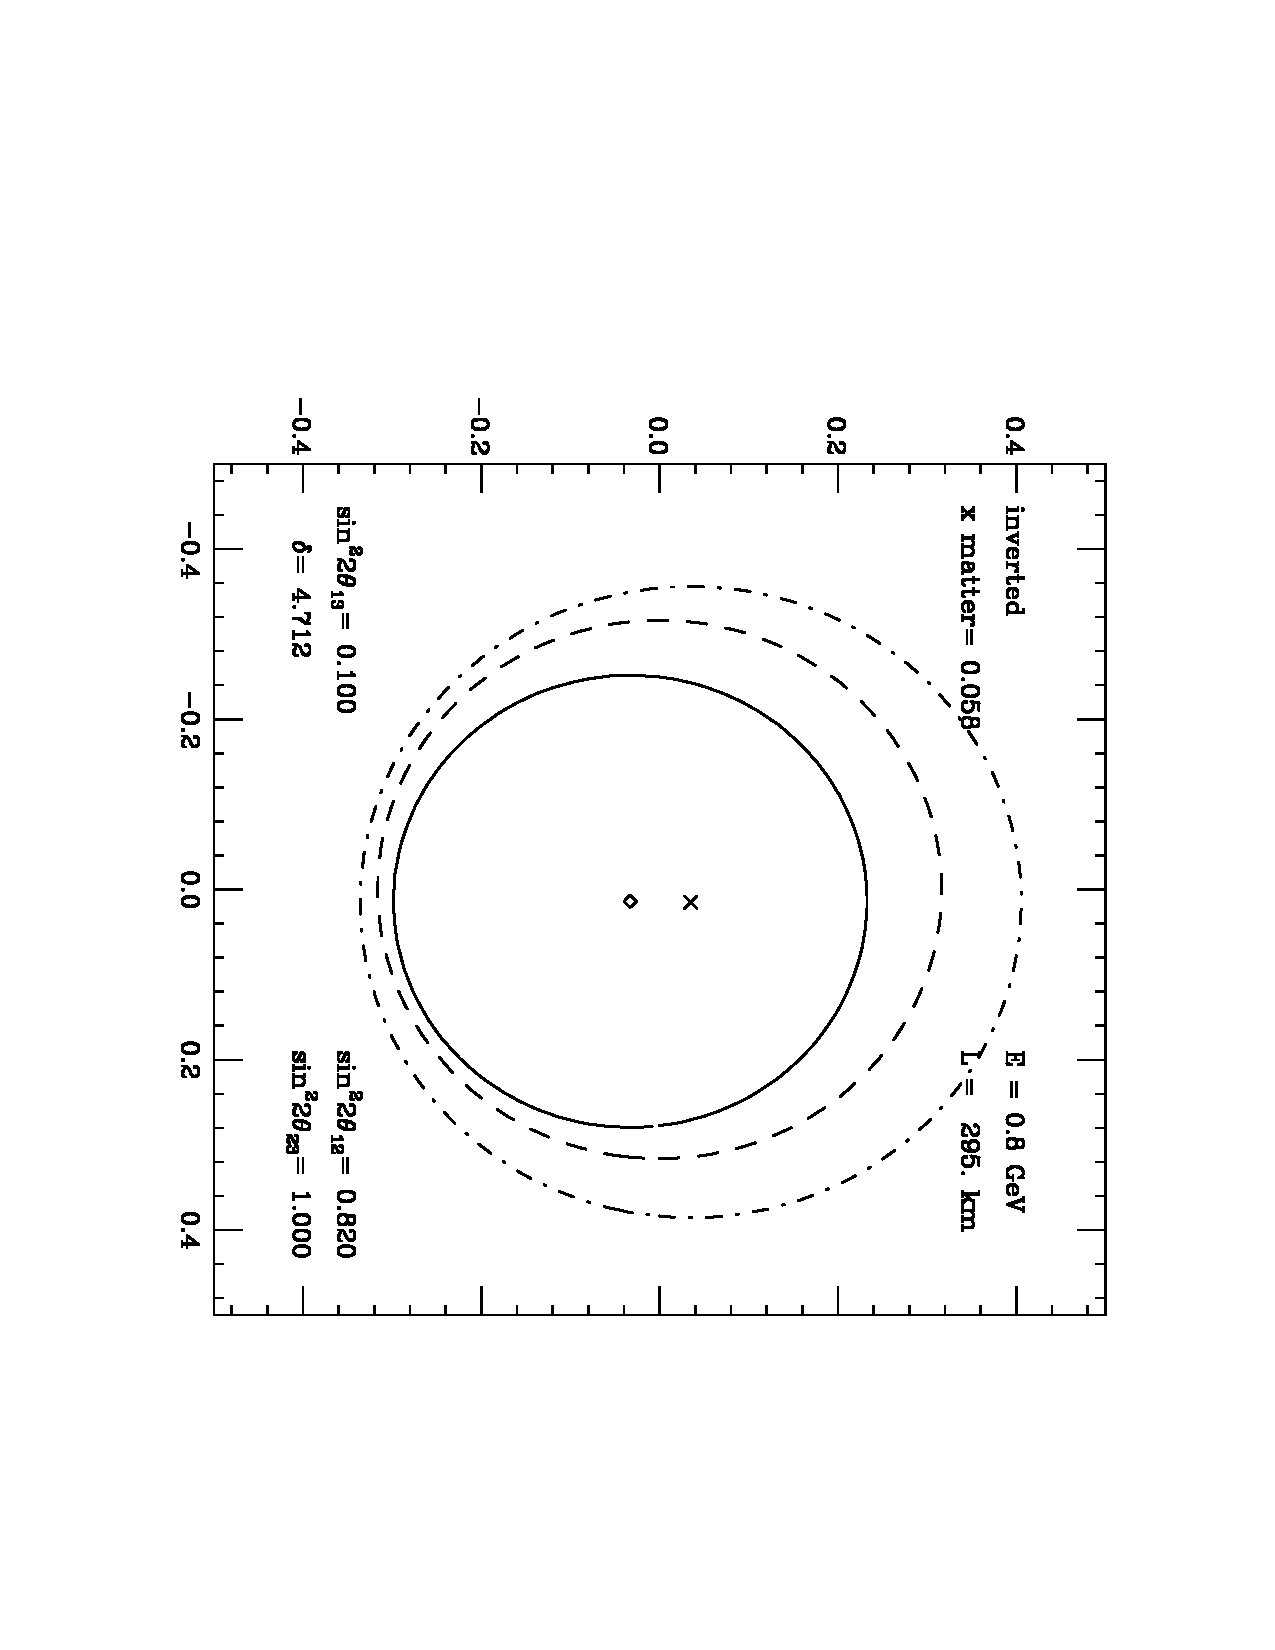
\includegraphics[width=2.75in,angle=90]{RNC/cpv_t2k_threepibytwo_inv.pdf}
\caption{ Plots for T2K.  Upper, with true hierarchy being normal, with $\delta_{CP}=\pi/2$.  Lower, again with true hierarchy being normal, but now with $\delta_{CP}=3\pi/2$. The dot dash circles show the constraints from $\nu_\mu$ scattering, while the solid circles are for $\nubar_\mu$.  The dashed circles show the constraints from a hypothetical perfect measurement of $\sin^22\theta_{13}$.\label{fig_four}}
\end{center}\end{figure}

\subsubsection{\NOvA}


\NOvA\ uses an off-axis beam, which is rather monochromatic.  The far detector has a mass of 14 kt and is located at Ash River, Minnesota, 810 km from the beam source at Fermilab.  The experiment is scheduled to take data starting in 2014 and to run for six years.  In addition to the far detector, there is a 330-t near detector.   The \NOvA\ website describes the detectors as being ``made up of 344,000 cells of extruded, highly reflective plastic PVC filled with liquid scintillator. Each cell in the far detector measures 3.9 cm wide, 6.0 cm deep and 15.5 meters long.'' 
 Fig.~\ref{fig_two} shows the statistical separation power of \NOvA; we see that the separation is easiest when $\delta_{CP}\approx 3\pi/2.$   
The reach as determined by the \NOvA\ collaboration is shown in Fig.~\ref{fig_seven}.
These figures are consistent with Fig.~\ref{fig_two} and show that 
for about a third of a range of $\delta_{CP}$, centered around
 $\delta_{CP}=3\pi/2$, \NOvA\ can determine the hierarchy with a
 confidence of $2-3\sigma$. A combination of \NOvA\ and T2K
 (Fig.~\ref{fig_seven}, right) has an ability to resolve the hierarchy at
 $1-3\sigma$ significance for all values of $\delta_{CP}$. This comes
 about because of the difference in baselines: T2K is primarily
 sensitive to the CP asymmetry between neutrinos and antineutrinos
 (effect of $\delta_{CP}$), which can be subtracted from the \NOvA\
 asymmetries to extract the matter-induced hierarchy signal. 

\subsubsection{Prospects}

\NOvA\ has a much better chance of measuring the hierarchy than T2K, but this
would only be possible for a very favorable value of $\delta_{CP}$.
It could find an indication of the hierarchy and this could reduce the
impact of later experiments if they ended up confirming, say, a
two-sigma \NOvA\ result.   
The sensitivity of T2K and \NOvA\ could be improved with additional run
time, or upgrades to the detectors or the beam
intensity~\cite{atm:Winter}. 


\begin{figure}\begin{center}
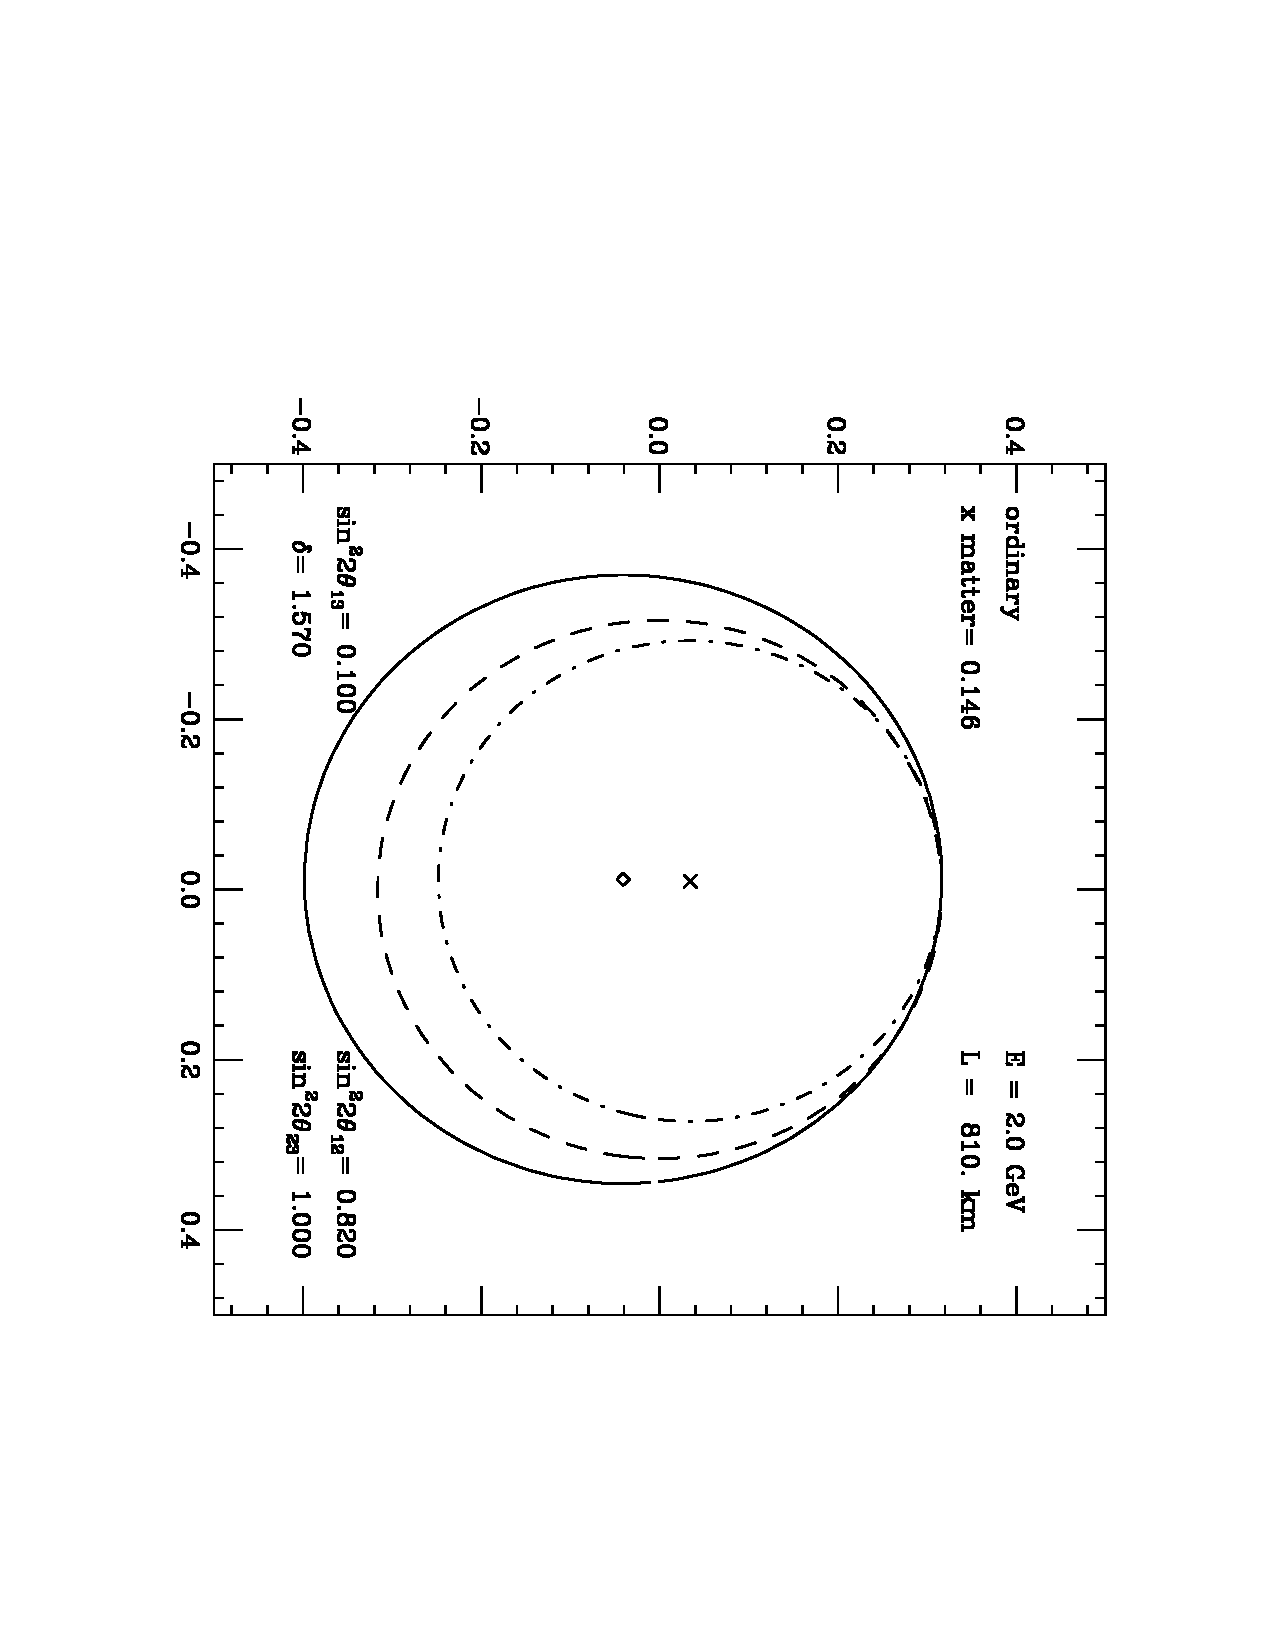
\includegraphics[width=2.75in,angle=90]{RNC/cpv_nova_pibytwo.pdf}
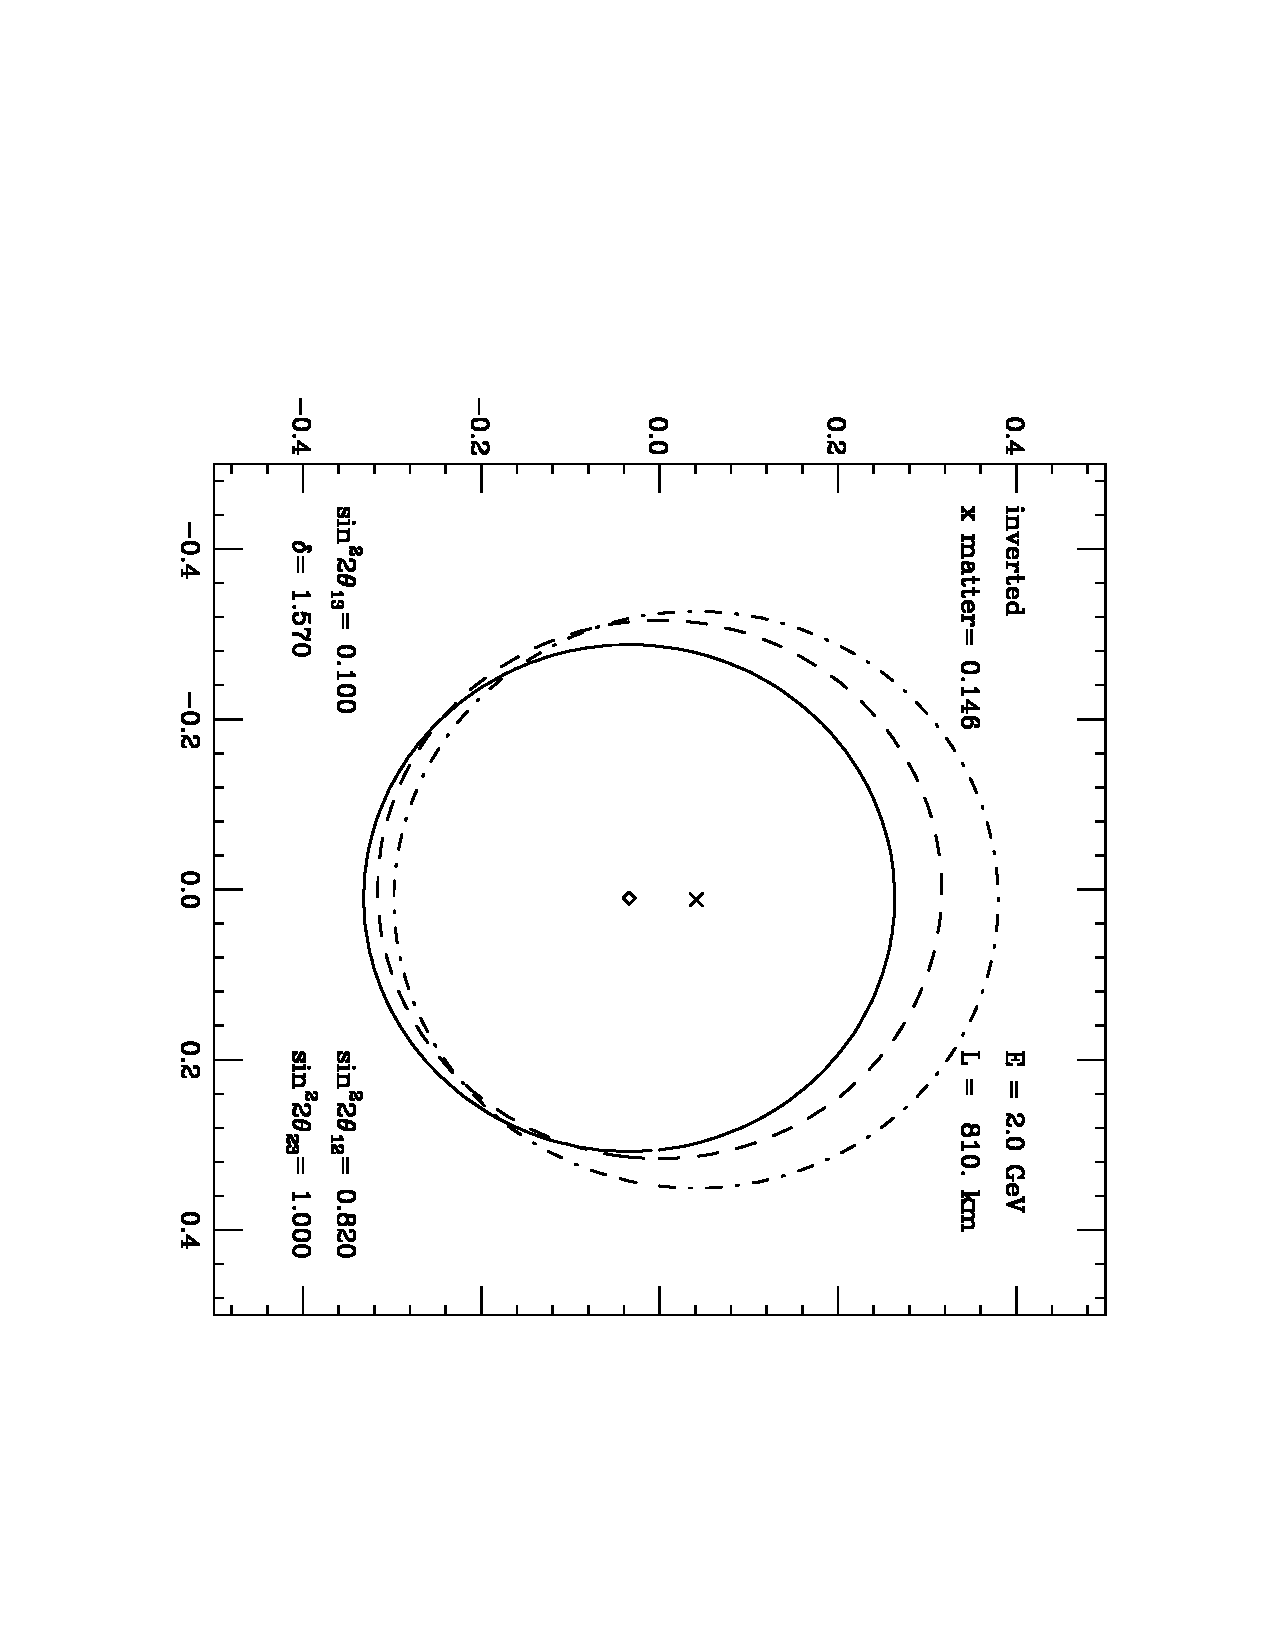
\includegraphics[width=2.75in,angle=90]{RNC/cpv_nova_pibytwo_inv.pdf}

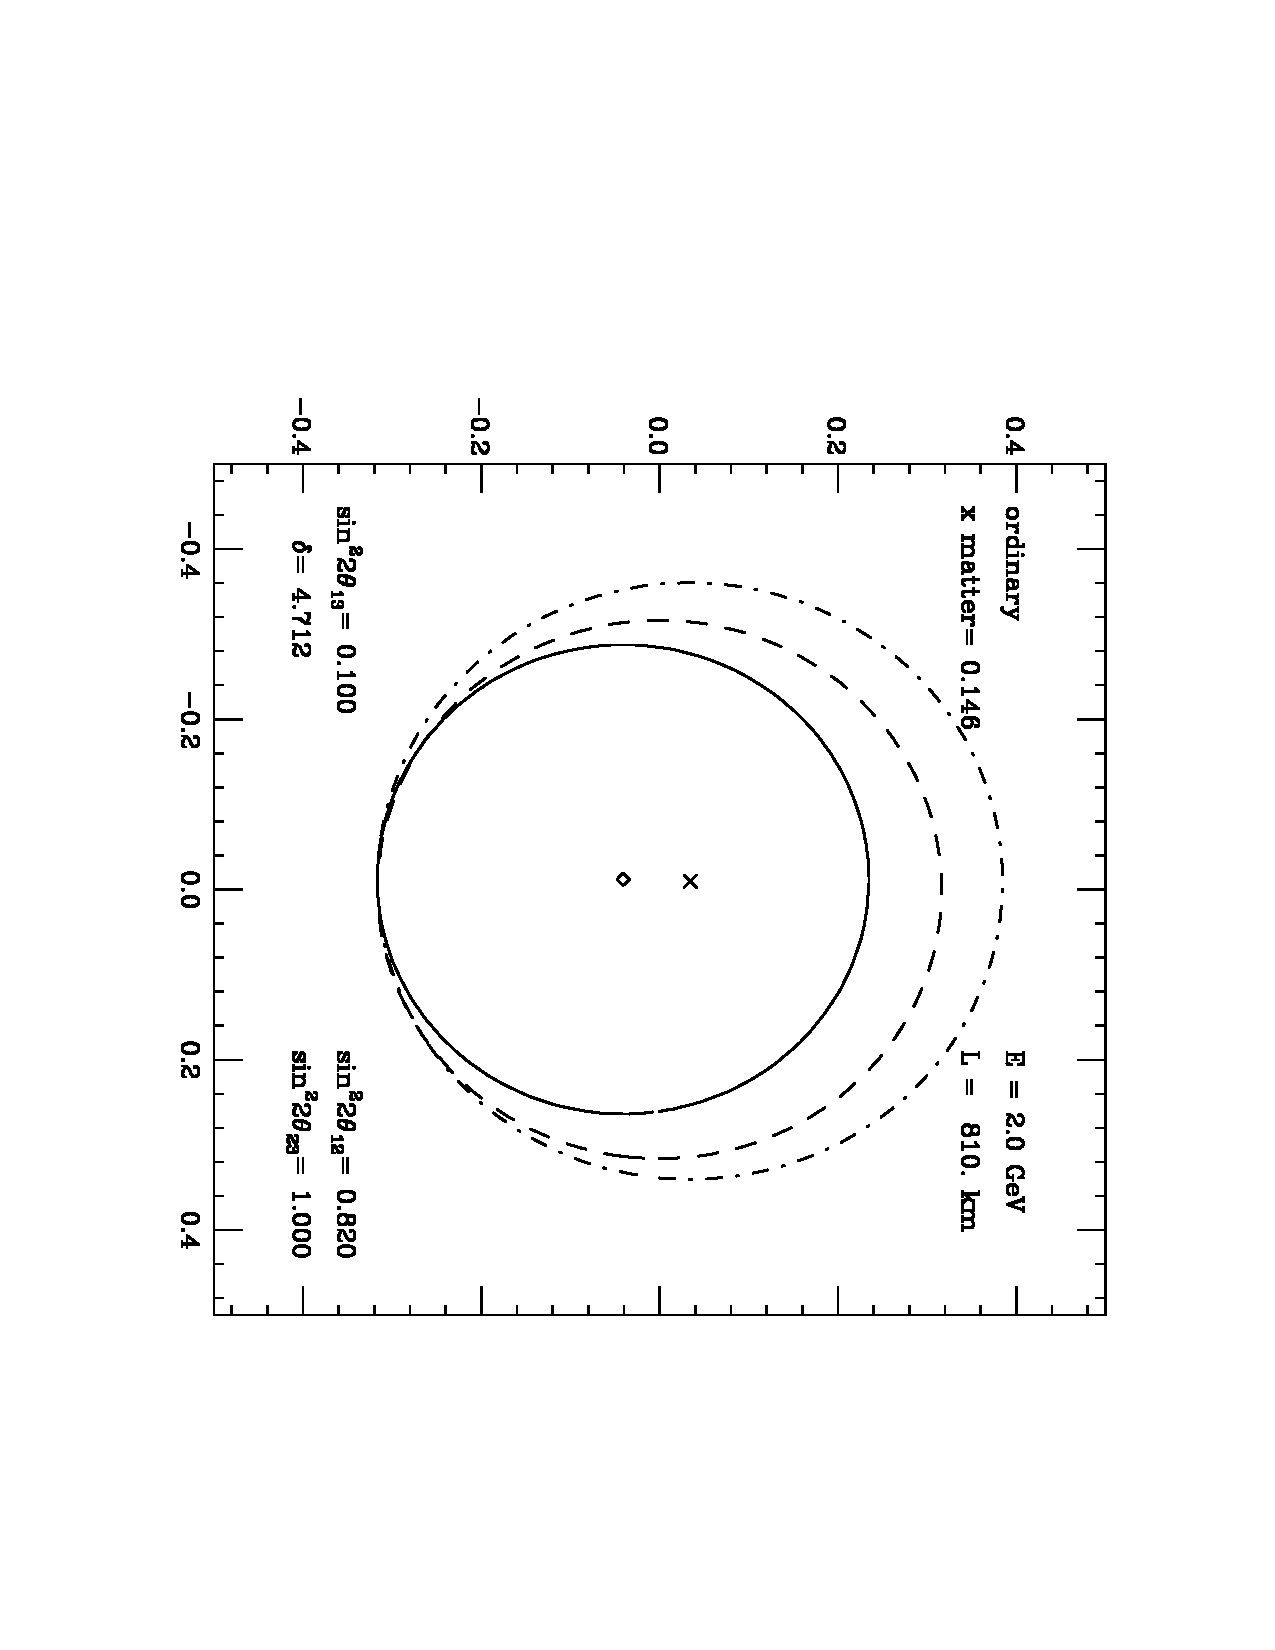
\includegraphics[width=2.75in,angle=90]{RNC/cpv_nova_threepibytwo.pdf}
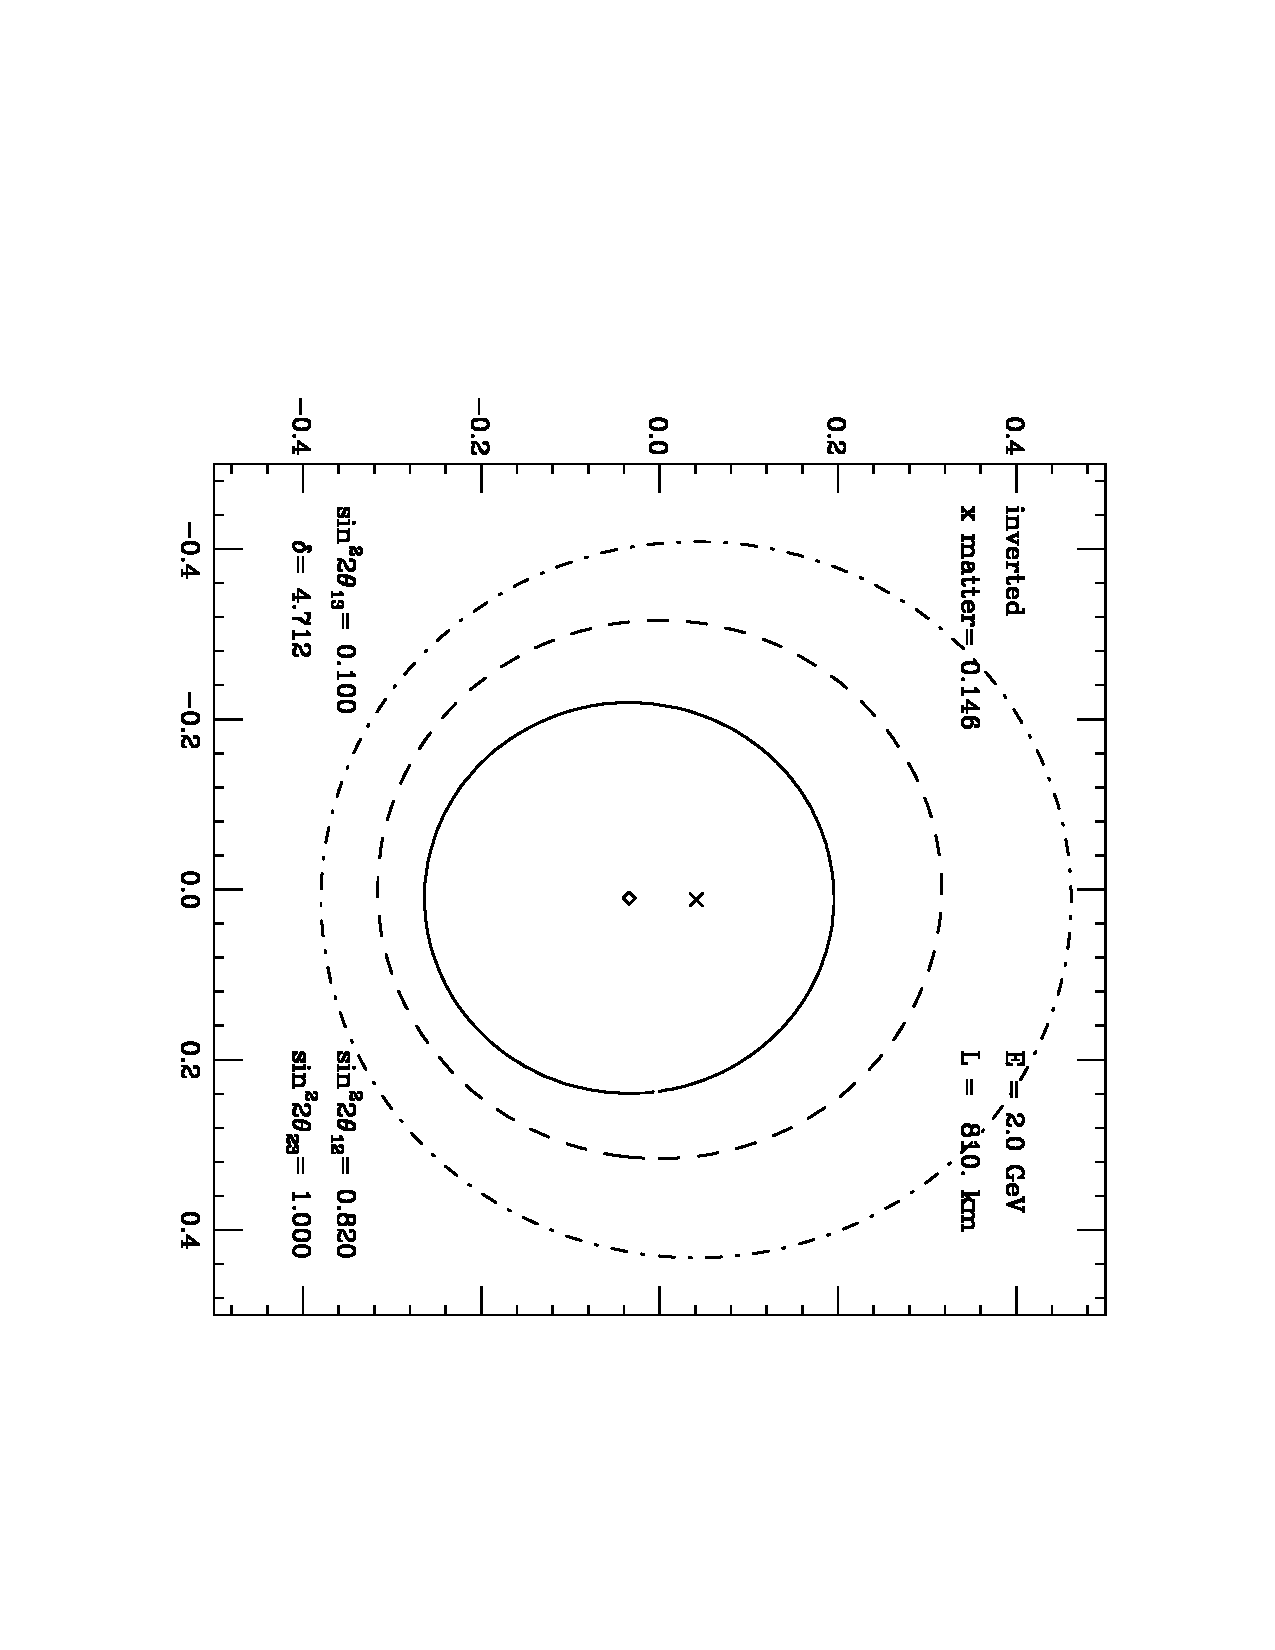
\includegraphics[width=2.75in,angle=90]{RNC/cpv_nova_threepibytwo_inv.pdf}
\caption{Plots for \NOvA.  Upper, with true hierarchy being normal, with $\delta_{CP}=\pi/2$.  Lower again,  with true hierarchy being normal, but now with $\delta_{CP}=3\pi/2$. The dot dash circles show the constraints from $\nu_\mu$ scattering, while the solid circles are for $\nubar_\mu$. The dashed circles show the constraints from a hypothetical perfect measurement of $\sin^22\theta_{13}$\label{fig_two}}
\end{center}
\end{figure}
\clearpage

\begin{figure}\begin{center}
%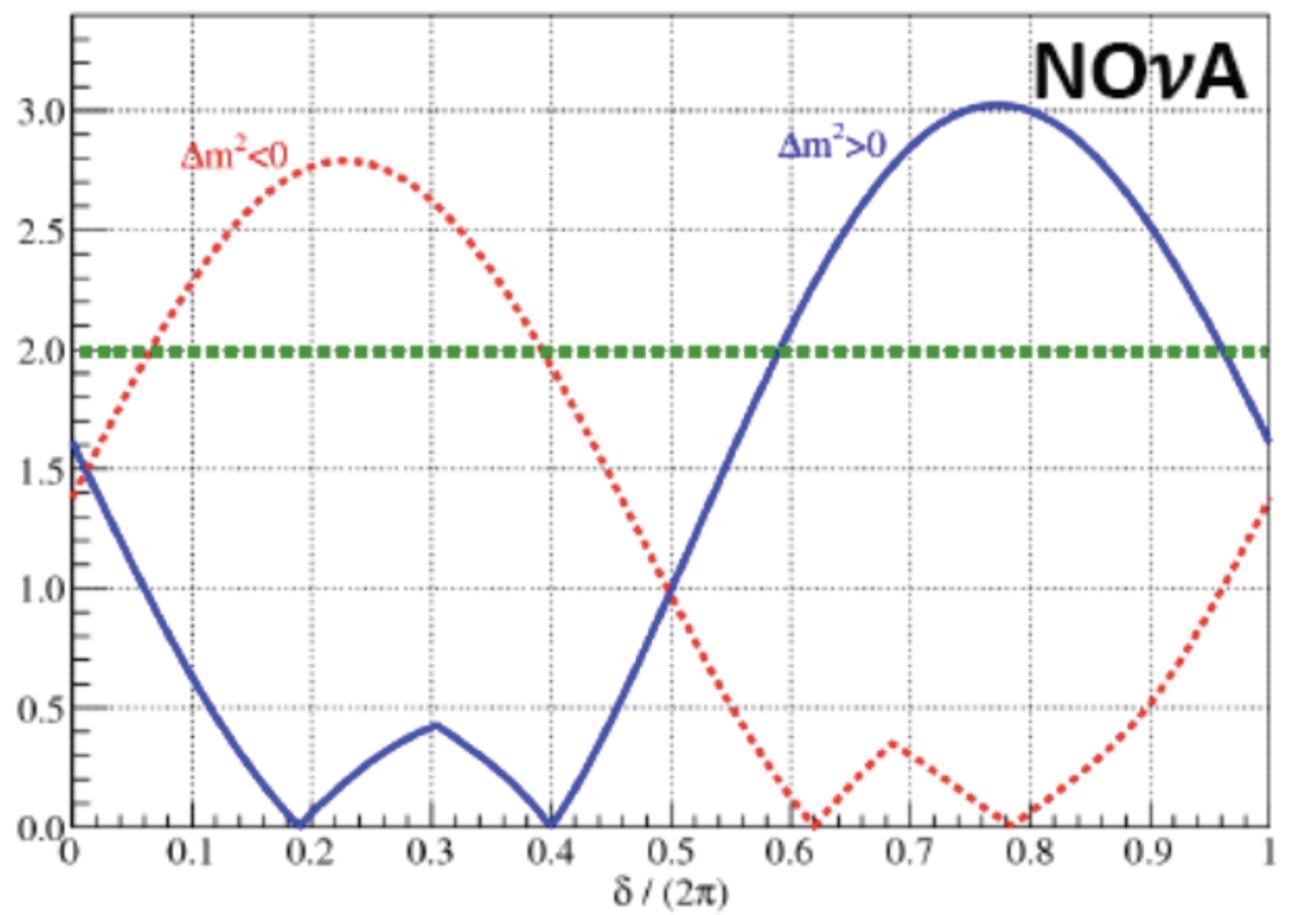
\includegraphics[width=0.42\textwidth]{RNC/novaalone.pdf}
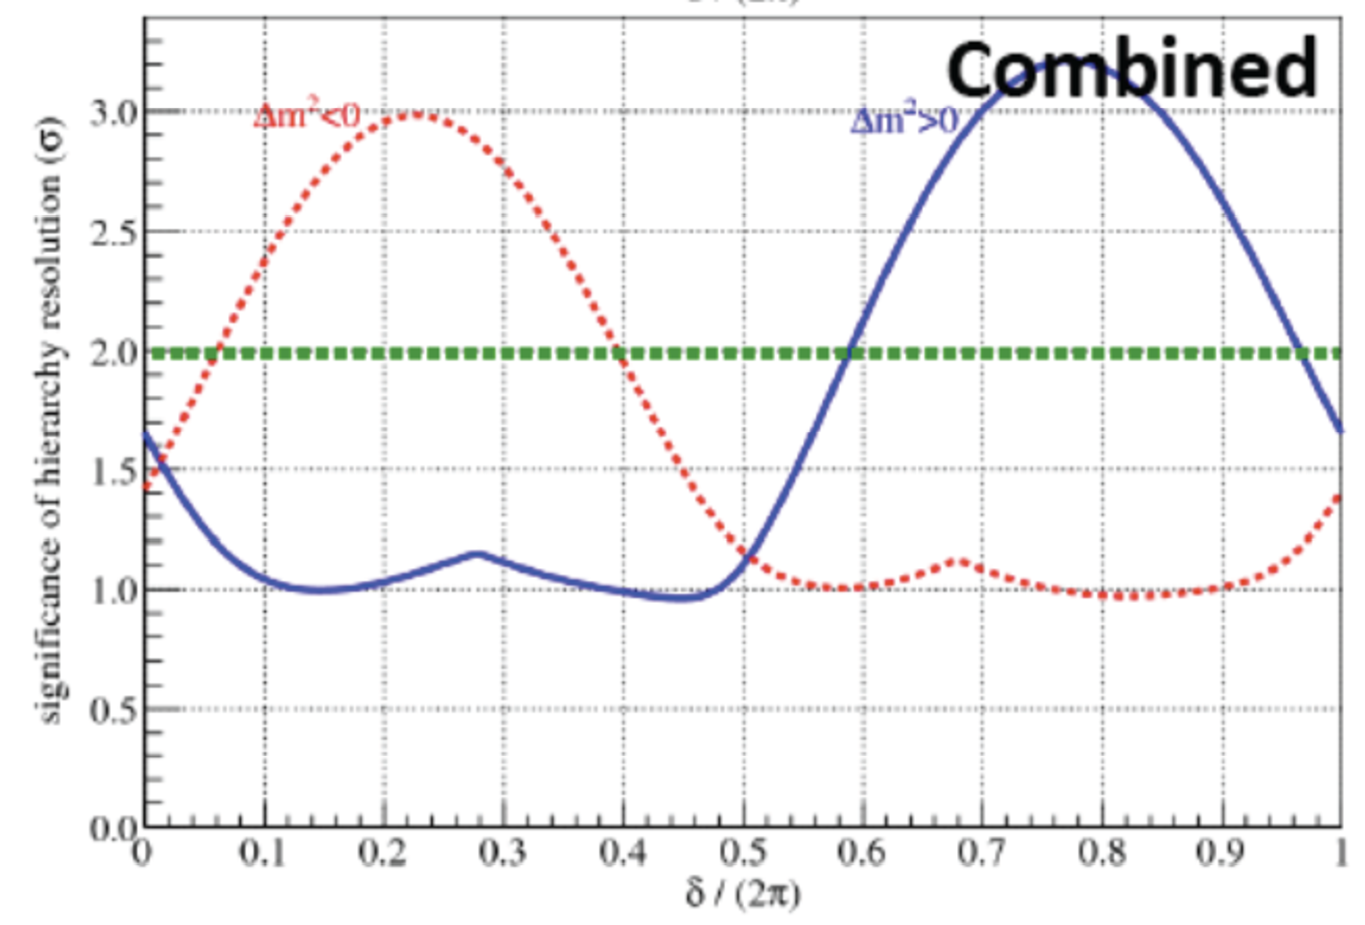
\includegraphics[width=0.44\textwidth]{RNC/t2knova.pdf}
\caption{Significance with which (Left) \NOvA\ and (Right) T2K+\NOvA\ can resolve the mass hierachy for  $\sin^22\theta_{13}=0.095$ and $\sin^22\theta_{23}=1$, as a function of $\delta_{CP}$. This assumes a nominal 3+3 year run plan. The blue/solid (red/dashed) curve shows the sensitivity given a normal (inverted) hierarchy. 
Figures from \NOvA\ document \cite{patterson}. \label{fig_seven}}
\end{center}
\end{figure}



